\documentclass[10pt,a4paper]{article}
\usepackage[utf8]{inputenc}
\usepackage{amsmath}
\usepackage{amsfonts}
\usepackage{amssymb}
\usepackage{graphicx}
\author{Pranav Satheesh}
\title{Relativity Assignments}
\begin{document}
\maketitle

\section{Einstein's velocity addition}

In this problem, you will derive the velocity addition rule in relativity using Lorentz transformations. Consider a particle A in the frame B. Her velocity w.r.t frame B is $V_{AB}$. In another frame C moving w.r.t B with a velocity $V_{CB}$. Show that the velocity of A w.r.t to the frame C using \textbf{Lorentz transformation}:

\begin{equation}
V_{AC} = \frac{V_{AB} + V_{BC}}{1 + (V_{AB} V_{BC} / c^2)}
\end{equation}

(\textit{\textbf{Hint} : You can use consider the velocity to be $u =\frac{dx}{dt}$ in the frame B and then write the lorentz transformation equations for $dx$ and $dt$ to the frame C where these become $\bar{dx}$ and $\bar{dt}$})

\section{Superluminal Motion}
Astronomers observed radio galaxies moving with velocities exceeding the velocity of c!
M87 is an example in the Virgo cluster
The distance to this galaxy, M87, is about D = 62 million light years. One can use this distance to convert angular separations into linear separations across the line of sight. 


\begin{figure}[htbp]
\centering
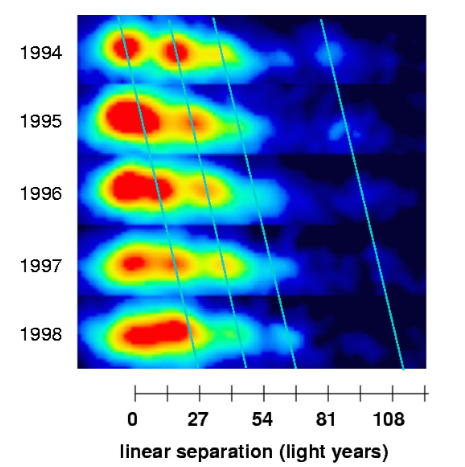
\includegraphics[scale=0.3]{lumino.png} 
\caption{Blobs}
\end{figure}

\begin{enumerate}
 \item Now, look at one of the blobs: the innermost one, which appears most clearly in 1996 and 1997. Approximately calculate the velocity of the blob.Hold on a minute! Is this against special relativity postulate 2 ?
 \item This calculation is not correct. The clouds are actually movng traight towards us with a velocity below c. As the cloud rapidly approaches, the distance light has to travel reduces and hence it would appear to reach us sooner. This effect can be understood from the second diagram. The cloud stars at N and moves at an angle $\theta$ w.r.t the line of sight of the observer O. Let $\vec{V}$ be the velocity of the cloud and let $t_{obs}$ be the time the observer sees the light emitted from the cloud at time $t$. From the distance travelled by light calculare the  relation between $t_{obs}$ and $t$.
 
\begin{figure}[htbp]
\centering
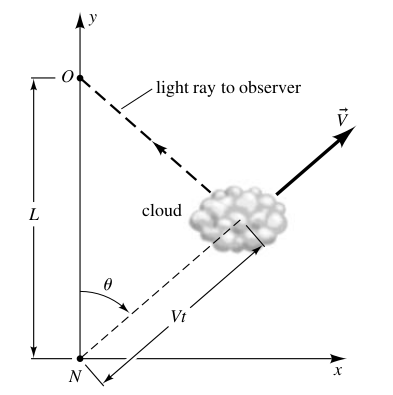
\includegraphics[scale=0.5]{superlum2.png} 
\caption{Apparent motion of the cloud}
\end{figure} 
 
\item Now we using the $t_{obs}$ relation, figure out the transverse speed $V_{T}$ observed by the observer using $V_{T} = dx/d t_{obs}$. 
\item Can you now plot $V_{T}$ for different $\theta$ and see at what angles you see an apparent motion greater than c ?
 
 
\end{enumerate}



\section{Relativistic Doppler Effect}

In this exercise you will derive the Doppler effect using Lorentz transformations. 

Consider the source to be at rest and the reciever is moving away with some welovity $v$ and $v>0$. Use suscript $s$ for source and $r$ for reciever.

\begin{enumerate}
\item Consider the first pulse recieved by the recieber at $t_s = 0$ and $x_s = 0$. $\lambda_s$ is the wavelength of the wave. Now is time $t_{rs}$ the reciever recieves the secon pulse. Then show that

$$ c t_{rs} = \lambda_s + v t_{rs} $$

\item We now need to make a lorentz transformation to reciever frame and change $t_{rs}$ to $t_{r}$. Show that after doing Lorentz transformation

$$ t_{r} = \frac{t_{rs}}{\gamma}$$

\item Now subsitiute this in the previous relation and obtain the fampus relation between the frequencies.

$$ f_{r} = \sqrt{\frac{1- \frac{v}{c}}{1+ \frac{v}{c}}} f_{s} $$

\end{enumerate}

\end{document}

